\documentclass[compress]{beamer}
\mode<presentation>
\usetheme{Warsaw}
\usecolortheme{seagull}
%\useoutertheme[subsection=false]{smoothbars}
\useoutertheme{infolines}
\useinnertheme{rectangles}

\usepackage{array}
\usepackage{amsmath,amssymb,amsfonts,mathrsfs,amsthm}
\usepackage[utf8]{inputenc}
\usepackage{listings}
\usepackage{mathtools}
\usepackage{dsfont}
\usepackage{pdfpages}
\usepackage[textsize=footnotesize,color=green]{todonotes}
\usepackage{algorithm, algorithmic}
\usepackage{bm}
\usepackage{tikz}
\usepackage[normalem]{ulem}

\usepackage{graphicx}
\usepackage{subfigure}
\usepackage{color}
\usepackage{undertilde}
\usepackage{pdflscape}
\usepackage{pifont}

\renewcommand{\topfraction}{0.85}
\renewcommand{\textfraction}{0.1}
\renewcommand{\floatpagefraction}{0.75}

\newcommand{\vect}[1]{\ensuremath\boldsymbol{#1}}
\newcommand{\tensor}[1]{\underline{\vect{#1}}}
\newcommand{\del}{\triangle}
\newcommand{\grad}{\nabla}
\newcommand{\curl}{\grad \times}
\renewcommand{\div}{\grad \cdot}
\newcommand{\ip}[1]{\left\langle #1 \right\rangle}
\newcommand{\eip}[1]{a\left( #1 \right)}
\newcommand{\pd}[2]{\frac{\partial#1}{\partial#2}}
\newcommand{\pdd}[2]{\frac{\partial^2#1}{\partial#2^2}}

\newcommand{\circone}{\ding{192}}
\newcommand{\circtwo}{\ding{193}}
\newcommand{\circthree}{\ding{194}}
\newcommand{\circfour}{\ding{195}}
\newcommand{\circfive}{\ding{196}}

\newcommand{\Reyn}{\rm Re}

\newcommand{\bs}[1]{\boldsymbol{#1}}
\DeclareMathOperator{\diag}{diag}

\newcommand{\equaldef}{\stackrel{\mathrm{def}}{=}}

\newcommand{\tablab}[1]{\label{tab:#1}}
\newcommand{\tabref}[1]{Table~\ref{tab:#1}}

\newcommand{\theolab}[1]{\label{theo:#1}}
\newcommand{\theoref}[1]{\ref{theo:#1}}
\newcommand{\eqnlab}[1]{\label{eq:#1}}
\newcommand{\eqnref}[1]{\eqref{eq:#1}}
\newcommand{\seclab}[1]{\label{sec:#1}}
\newcommand{\secref}[1]{\ref{sec:#1}}
\newcommand{\lemlab}[1]{\label{lem:#1}}
\newcommand{\lemref}[1]{\ref{lem:#1}}

\newcommand{\mb}[1]{\mathbf{#1}}
\newcommand{\mbb}[1]{\mathbb{#1}}
\newcommand{\mc}[1]{\mathcal{#1}}
\newcommand{\nor}[1]{\left\| #1 \right\|}
\newcommand{\snor}[1]{\left| #1 \right|}
\newcommand{\LRp}[1]{\left( #1 \right)}
\newcommand{\LRs}[1]{\left[ #1 \right]}
\newcommand{\LRa}[1]{\left\langle #1 \right\rangle}
\newcommand{\LRc}[1]{\left\{ #1 \right\}}
\newcommand{\tanbui}[2]{\textcolor{blue}{\sout{#1}} \textcolor{red}{#2}}
\newcommand{\Grad} {\ensuremath{\nabla}}
\newcommand{\Div} {\ensuremath{\nabla\cdot}}
\newcommand{\Nel} {\ensuremath{{N^\text{el}}}}
\newcommand{\jump}[1] {\ensuremath{\LRs{\![#1]\!}}}
\newcommand{\uh}{\widehat{u}}
\newcommand{\fnh}{\widehat{f}_n}
\renewcommand{\L}{L^2\LRp{\Omega}}
\newcommand{\pO}{\partial\Omega}
\newcommand{\Gh}{\Gamma_h}
\newcommand{\Gm}{\Gamma_{-}}
\newcommand{\Gp}{\Gamma_{+}}
\newcommand{\Go}{\Gamma_0}
\newcommand{\Oh}{\Omega_h}

\newcommand{\eval}[2][\right]{\relax
  \ifx#1\right\relax \left.\fi#2#1\rvert}

\def\etal{{\it et al.~}}


\def\arr#1#2#3#4{\left[
\begin{array}{cc}
#1 & #2\\
#3 & #4\\
\end{array}
\right]}
\def\vecttwo#1#2{\left[
\begin{array}{c}
#1\\
#2\\
\end{array}
\right]}
\def\vectthree#1#2#3{\left[
\begin{array}{c}
#1\\
#2\\
#3\\
\end{array}
\right]}
\def\vectfour#1#2#3#4{\left[
\begin{array}{c}
#1\\
#2\\
#3\\
#4\\
\end{array}
\right]}

\newcommand{\G} {\Gamma}
\newcommand{\Gin} {\Gamma_{in}}
\newcommand{\Gout} {\Gamma_{out}}

\title{A DPG method for compressible flow problems}
\author{Jesse Chan}

\begin{document}
\begin{frame}
\maketitle
\end{frame}

\section{Introduction/Literature review}
\frame{
\frametitle{Compressible flow problems}
\begin{figure}
\centering
\subfigure[Shock wave]{\includegraphics[scale=.0704]{figs/compFlowPics/bullet_shock.png}}
\subfigure[Boundary layer]{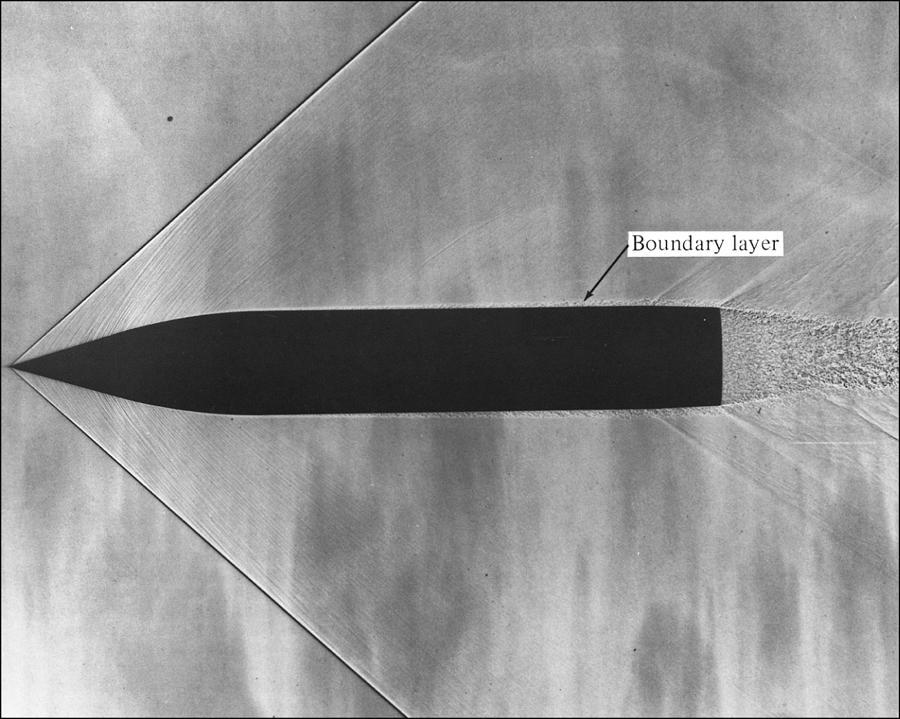
\includegraphics[scale=.16]{figs/compFlowPics/boundary_layer.png}}
%\subfigure{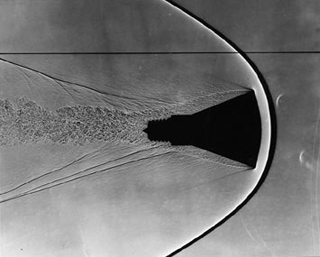
\includegraphics[scale=.15]{figs/compFlowPics/capsule.png}}
\end{figure}
Compressible flow plays an important role in the aerospace and energy industries - supersonic aircraft, combustion engines, etc. 

}
\frame{
\frametitle{Goal: Compressible Navier-Stokes equations}
\begin{columns}[c]
\begin{column}{.475\textwidth}
Numerical difficulties:
\begin{itemize}
\item{} Resolving solutions (sharp, localized $O(\Reyn^{-1})$ phenomena)
\begin{itemize}
\item{} Shocks, boundary layers
\item{} Turbulent phenomena
\end{itemize}
\item{} Stability of numerical schemes
\begin{itemize}
\item{} Coarse/adaptive grids
\item{} Higher order
\end{itemize}
\end{itemize}
\end{column}
\begin{column}{.475\textwidth}
\begin{figure}
\centering
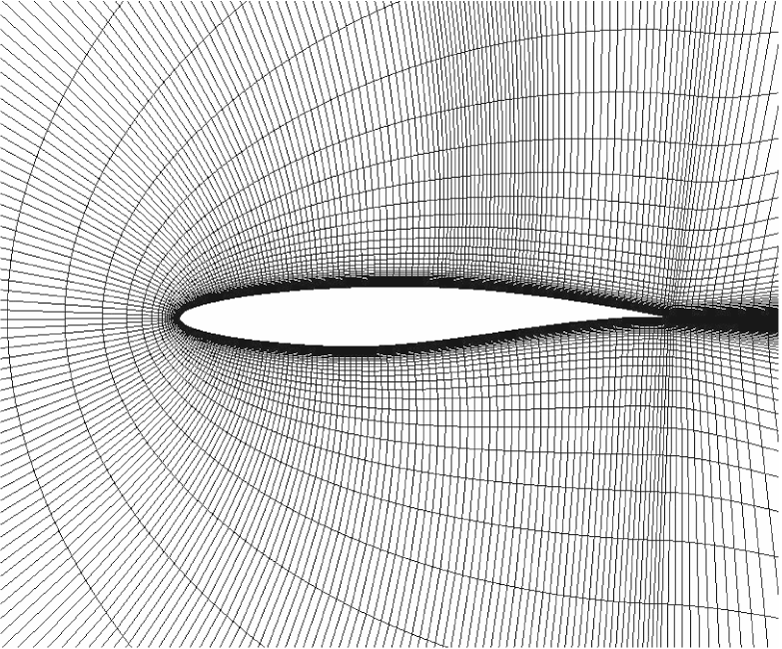
\includegraphics[scale = .7]{figs/compFlowPics/airfoil_mesh.png}
\end{figure}
\end{column}
\end{columns}
\vspace{1cm}
\begin{center}
Idea: begin first with the model problem of convection-diffusion.
\end{center}
}
\frame{
\frametitle{Convection-diffusion as a model problem}
\[
\div \left(\beta u\right) - \epsilon \Delta u = f, \quad \text{on }\Omega \in \mathbb{R}^3
\]
}
\frame{
\frametitle{Dealing with stability/robustness}
Convection-diffusion equation in 1D is $\beta u' - \epsilon u'' = f$.
%\vspace{-.5cm}
\begin{columns}[c]
\begin{column}{.49\textwidth}
Standard continuous Galerkin variational formulation: solve
\[
b(u,v) = l(v) 
\]
where
\begin{align*}
b(u,v) &= \int_\Omega -\beta uv' + \epsilon u'v' \\
l(v) &= \int_\Omega f v 
\end{align*}
\end{column}
\begin{column}{.49\textwidth}
\begin{figure}
\centering
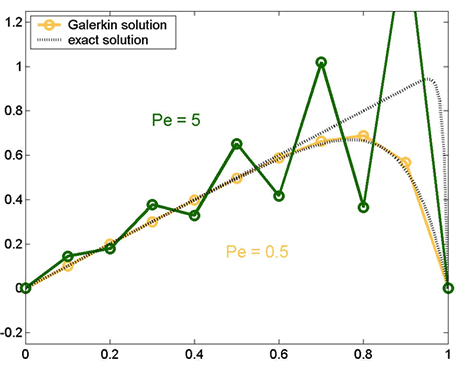
\includegraphics[scale=.3]{figs/GalerkinOscTight.png}
\caption{Oscillations in the standard Galerkin method for underresolved meshes and small $\epsilon$.}
\end{figure}
\end{column}
\end{columns}
}
\frame{
Historical stabilization methods: 
\begin{itemize}
\item Artificial diffusion - solve
\[
\beta u' - \tilde{\epsilon} u'' = f
\]
where $\tilde{\epsilon}$ is set depending on $\beta$, $\epsilon$, and the mesh. 
\item Upwind stencils - for positive $\beta$, and uniform grid points $x_A$,
\[
u'(x_A) \approx \frac{u_h(x_A)-u_h(x_{A-1})}{h}
\]
\end{itemize}

Both of these methods introduce additional numerical diffusion, and their effectiveness depends on the forcing $f$ and parameters $h$, $|\beta|$, and $\epsilon$.
}
\frame{
\frametitle{Streamline-upwind Petrov-Galerkin (SUPG)}
SUPG solves $b_{\rm SUPG}(u,v) = l_{\rm SUPG}(v)$, where
\begin{align*}
b_{\rm SUPG}(u,v) &= b(u,v)+ \sum_{K} \int_{K} \tau \LRp{L_{\rm adv} v} L u \\
l_{\rm SUPG}(v) &= l(v) + \sum_{K} \int_{K} \tau \LRp{L_{\rm adv}v} f.
\end{align*}
\vspace{-.5cm}
\begin{columns}[c]
\begin{column}{.47\textwidth}
\vspace{-.5cm}
\begin{itemize}
\item{} $L_{\rm adv}u = \div \left(\beta u\right)$, and $\tau$ is a parameter. 
\item{} Recovers ``exact'' artificial diffusion for $f=0$.
\item{} Effective for $f\neq 0$, unlike ``exact'' artificial diffusion.
\item{} \emph{Residual-based} stabilization. 
\end{itemize}
\end{column}
\begin{column}{.52\textwidth}
\begin{figure}
\centering
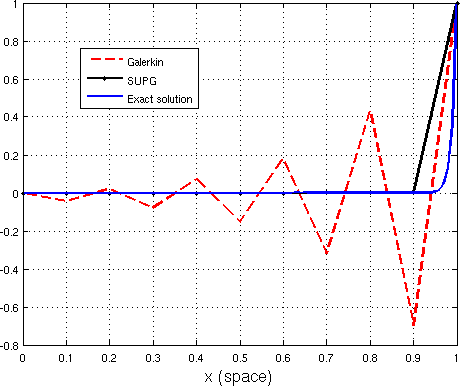
\includegraphics[scale=.3]{figs/SUPG.png}
\caption{Exact, FEM, and SUPG solutions.}
\end{figure}
\end{column}
\end{columns}
}

\frame{
Can be interpreted as a \emph{Petrov-Galerkin} method,
\[
b\LRp{u,\tilde{v}_{i}} = l\LRp{\tilde{v}_{i}}, \quad \forall i = 1,\ldots,N-1,
\]
where the SUPG test function $\tilde{v}_{i}$ is defined elementwise as
\[
\tilde{v}_{i} = \phi_i(x) + \tau L_{\rm adv} \phi_i.  
\]
\begin{figure}
\centering
\subfigure{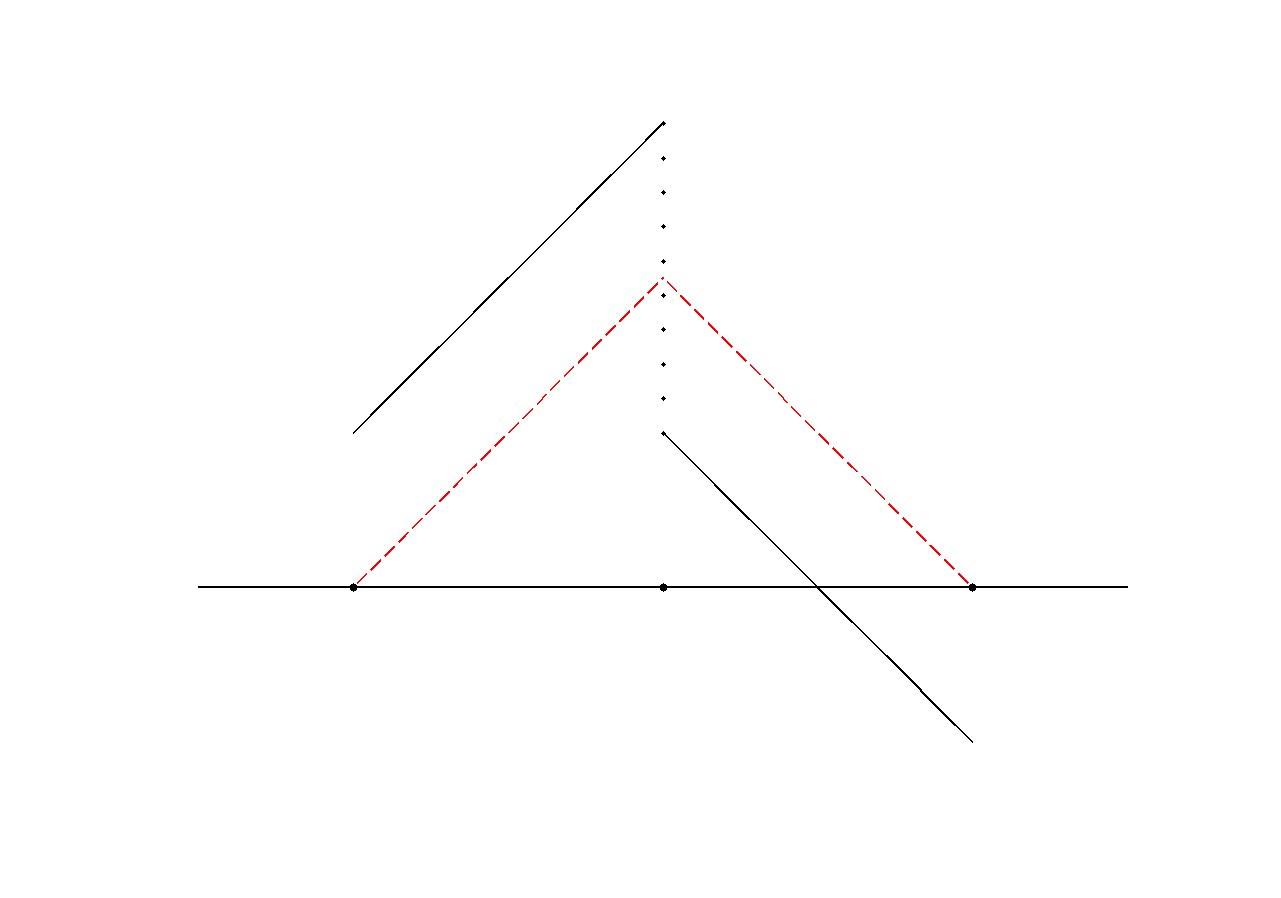
\includegraphics[scale=.185]{figs/SUPGtest.png}}
\caption{SUPG test function $v_i$.}
\end{figure}
}

\section{The DPG Method}
\frame{
\frametitle{Minimum residual methods through optimal testing}
Identify $B:U\rightarrow V'$ such that
\[
\langle Bu,v\rangle_V \coloneqq b(u,v), \quad u\in U, v\in V.
\]
Then, $b(u_h,v) = l(v)$ is equivalent to the equation in $V'$
\[
Bu_h = l
\]
We seek to minimize the functional on $V'$
\[
J(u_h) = \frac{1}{2}\|Bu_h-l\|_{V'}^2 \coloneqq\frac{1}{2} \sup_{v\in V\setminus\{0\}} \frac{| b(u_h,v)-l(v)|^2}{\nor{v}_V^2}.
\]
}

\frame{
Let $R_V: V \to V'$ be the isometric the Riesz map st.\
\[
\langle R_V v,\delta v\rangle_V \coloneqq(v, \delta v)_V, \quad \forall \delta v \in V.
\]
Then, our functional $J(u_h)$ is equal to
\begin{equation*}
\min_{u_h\in U_h} J(u_h) = \frac{1}{2}\left\|Bu_h-l\right\|_{V'}^2 =  \frac{1}{2}\left\|R_V^{-1}(Bu_h-l)\right\|_V^2.
\end{equation*}
First order optimality: G\^ateaux derivative is zero in all directions $\delta u \in U_h$
\begin{align*}
\left(R_V^{-1}(Bu_h-l),R_V^{-1}B\delta u\right)_V = 0, \quad \forall \delta u \in U. 
\end{align*}
}
\frame{
First order optimality: G\^ateaux derivative is zero in all directions $\delta u \in U_h$
\begin{align*}
\left(R_V^{-1}(Bu_h-l),R_V^{-1}B\delta u\right)_V &= 0,\\
\rightarrow \LRa{(Bu_h-l),R_V^{-1}B\delta u} &= 0, \\
\rightarrow b(u_h,R_V^{-1}B\delta u) - l(R_V^{-1}B\delta u) &= 0
\end{align*}
For $\delta u \in U$, we define the {\em optimal test function} $v_{\delta u}$
\begin{equation*}
v_{\delta u} \coloneqq R_V^{-1}B\delta u 
\end{equation*} 
such that $J(u_h)$ is minimized by the solution of
\[
b\LRp{u_h,v_{\delta u}} = l\LRp{v_{\delta u}}, \quad \forall \delta u \in U
\]
}
\frame{
\frametitle{Practical details of DPG}
\begin{itemize}
\item By choosing $V$ as a \emph{broken} test space, test functions can be determined locally.
\item In practice, $V \coloneqq V_h$, where $\dim(V_h) > \dim(U_h)$ elementwise, and test functions are approximated via solving
\[
\LRp{v_{\delta u},\delta v}_V = b(\delta u,\delta v).
\]
\end{itemize}
}

\frame{
\frametitle{Properties of DPG}
\begin{itemize}
\item Symmetric positive-definite stiffness matrix
\item DPG provides best approximation in energy norm 
\[
\|u\|_E = \|Bu\|_{V'} = \sup \frac{b(u,v)}{\nor{v}_V}.
\]
\item Actual energy error is computable through the residual
\[
\nor{u-u_h}_E = \nor{B(u-u_h)}_{V'} = \nor{R_V^{-1}(l-Bu_h)}_V = \nor{e}_V
\]
where $(e,\delta v)_V = l(v)-b(u_h,v)$ for all $v\in V$. 
\end{itemize}
}

%\frame{
%\frametitle{Duality of norms}
%Duality of norms: for any trial norm $\nor{u}_U$,
%\[
%\nor{u}_{U} = \sup_{v \in V}\frac{b\LRp{u,v}}{\nor{v}_{V,U}}, \quad \nor{v}_{V,U} = \sup_{u \in U}\frac%{b\LRp{u,v}}{\nor{u}_{U}}.
%\]
%Likewise, for any test norm $\nor{v}_V$, 
%\[
%\nor{v}_{V} = \sup_{u \in U}\frac{b\LRp{u,v}}{\nor{U}_{U,V}}, \quad \nor{u}_{U,V} = \sup_{v \in V}\frac%{b\LRp{u,v}}{\nor{v}_{V}}.
%\]
%
%}

\frame{
\frametitle{Ultra-weak formulation}
Given a first order system of equations $Au = f$, we identify the \emph{partition} $\Oh$ and \emph{mesh skeleton} $\Gh$
\[
\Oh = \cup_{j=1}^\Nel K_j, \quad \Gh = \cup_{j=1}^\Nel \partial K_j
\]
The ultra-weak formulation for $Au = f$ on $\Oh$ is
\[
b\left(\left(u, \widehat{u}\right),v\right) \coloneqq \langle \widehat{u}, \jump{v}
\rangle_{\Gh} - (u,A_h^*v)_{\Oh}= \LRp{f,v}_{\Oh}.
\]
where
\[
u\in L^2\LRp{\Oh} \equiv L^2(\Omega), \quad v\in V=D(A^*_h), \quad
\widehat{u}\in \gamma(D(A)),
\]
where $D(A_h^*)$ is the broken graph space of $A_h^*$, and $\gamma(D(A))$ the trace space of the graph space of operator $A$.
}

\frame{
\frametitle{Canonical norms for the ultra-weak formulation}
Under the ultra-weak formulation, we have the following relations:
\begin{figure}[!h]
\centering
\begin{tabular}{l c c}
Trial norm & & Test norm \\
\hline
$\boxed{\|u\|^2_{\L} + \|\widehat{u}\|^2}$ & $\Longrightarrow$  & $\|A_h^*v\|_{\L}^2
+\left(\sup_{\widehat{u}} \frac{\LRa{ \widehat{u},
  \jump{v} }_{\Gh}}{\|\widehat{u}\|}\right)^2$ \\
%\hline
%Quasi-optimal trial norm & & Canonical test norm \\
%\hline
$\nor{u}_{\L}^2+\sup_{v } \left(\frac{\LRa{\widehat{u},
  \jump{v}}_{\Gh}}{\|v\|_V}\right)^2$ &  $\Longleftarrow$ & $\boxed{\|A_h^*v\|_{\L}^2 + \nor{v}_{\L}^2}$
\end{tabular}
\caption{The optimal \textit{test} norm is naturally derived by beginning with the canonical norm on the trial space, while the quasi-optimal \textit{trial} norm is derived from beginning with the canonical norm on the test space.}
\end{figure}
}

\section{A Robust DPG Method}

\frame{
\frametitle{Ultra-weak formulation for convection-diffusion}
In first order form, the convection-diffusion equation is
\[
A \LRp{u,\sigma} \coloneqq 
\LRs {
\begin{array}{c}
\div (\beta u - \sigma) \\ \frac{1}{\epsilon}\sigma - \grad u
\end{array}} = \LRs{
\begin{array}{c}
f \\ 0
\end{array}
}.
\]
The variational formulation is
\begin{align*}
b\left(\left(u,\sigma, \widehat{u}, \widehat{f}_n\right),
\left( v, \tau \right)\right) = \left(u,\div \tau - \beta \cdot \grad
v\right)_{\Oh} + \left(\sigma, \epsilon^{-1} \tau + \grad v\right)_{\Oh}&\\
 - \LRa{\jump{\tau\cdot n}, \widehat{u} }_{\Gh} + \LRa{ \widehat{f}_n,\jump{v} }_{\Gh}&,
\end{align*}
where $\widehat{f}_n \coloneqq \beta_n u - \sigma_n$. Note that $\div$ and $\grad$ are taken to act elementwise.
}

\frame{
\frametitle{Quasi-optimal norm under convection-diffusion}
For convection-diffusion, the quasi-optimal test norm is 
\[
\|\left(v,\tau\right)\|_V^2 = \| \div \tau - \beta \cdot \grad v
\|_{L^2}^2 + \| \epsilon^{-1} \tau + \grad v \|_{L^2}^2 +
\|v\|_{L^2}^2 + \|\tau\|_{L^2}^2.
\]
Problem with this test norm: approximability of test functions.
\vspace{-.3cm}
\begin{figure}[!h]
\centering
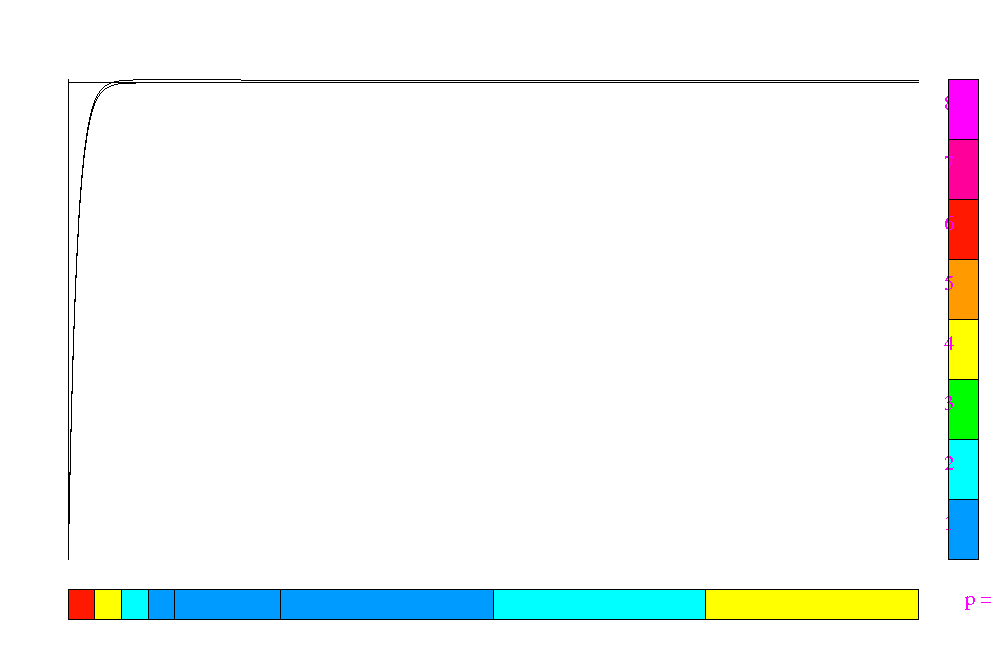
\includegraphics[scale=.175]{figs/opt.png}
\caption{$v$ and $\tau$ components of the 1D optimal test functions for flux $\widehat{f}_n$ on the \emph{right-hand} side of a unit element for $\epsilon = 0.01$. }
\label{fig:optTestBoundary}
\end{figure}
}

\frame{
\frametitle{Determining an alternative test norm}
``Necessary'' conditions for robustness --- let $\boldsymbol U = \LRp{u,\sigma,\widehat{u},\widehat{f}_n}$, then, by choosing specific $\LRp{v,\tau}$, 
\[
\nor{u}^2_{L^2(\Omega)} = b\LRp{{\boldsymbol U},\LRp{v,\tau}} = \frac{b\LRp{{\boldsymbol U},\LRp{v,\tau}}}{\nor{\LRp{v,\tau}}_V} \nor{\LRp{v,\tau}}_V \leq \nor{\boldsymbol U}_E \nor{\LRp{v,\tau}}_V
\]
If $ \nor{\LRp{v,\tau}}_V \lesssim \|u\|_{L^2(\Omega)}$, then we have the robust bound
\[
\nor{u}^2_{L^2(\Omega)} \lesssim \nor{\boldsymbol U}_E
\]
}

\frame{
\frametitle{Bilinear forms and induced adjoints}
Recall 
\begin{align*}
b\left(\left(u,\sigma, \widehat{u}, \widehat{f}_n\right),
\left( v, \tau \right)\right) = \left(u,\div \tau - \beta \cdot \grad
v\right)_{\Oh} + \left(\sigma, \epsilon^{-1} \tau + \grad v\right)_{\Oh}&\\
 - \LRa{\jump{\tau\cdot n}, \widehat{u} }_{\Gh} + \LRa{ \widehat{f}_n,\jump{v} }_{\Gh}&,
\end{align*}
We recover $\nor{u}_{L^2(\Omega)}$ by choosing continuous $\LRp{v,\tau}$ s.t.\
\begin{align*}
\div\tau - \beta \cdot \grad v   &= u\\
\frac{1}{\epsilon}\tau - \grad v &= 0
\end{align*}
where boundary conditions are s.t.\ $\LRa{\jump{\tau\cdot n}, \widehat{u} }_{\Gh}$ and $\LRa{ \widehat{f}_n,\jump{v} }_{\Gh}$ vanish. 
}

\frame{
\frametitle{``Building blocks'' norm}
Test norm quantities are robustly bounded from above by $\nor{u}_{L^2(\Omega)}$.  
\[
\|\left(v,\tau\right)\|_{V,K}^2 = \|v\|^2 + \epsilon \|\grad v\|^2 + \|\beta \cdot \grad v\|^2 + \| \div \tau\|^2 + \frac{1}{\epsilon}\|\tau\|^2.
\]
Problem: boundary layers in optimal test functions:
\begin{figure}[!h]
\centering
\subfigure{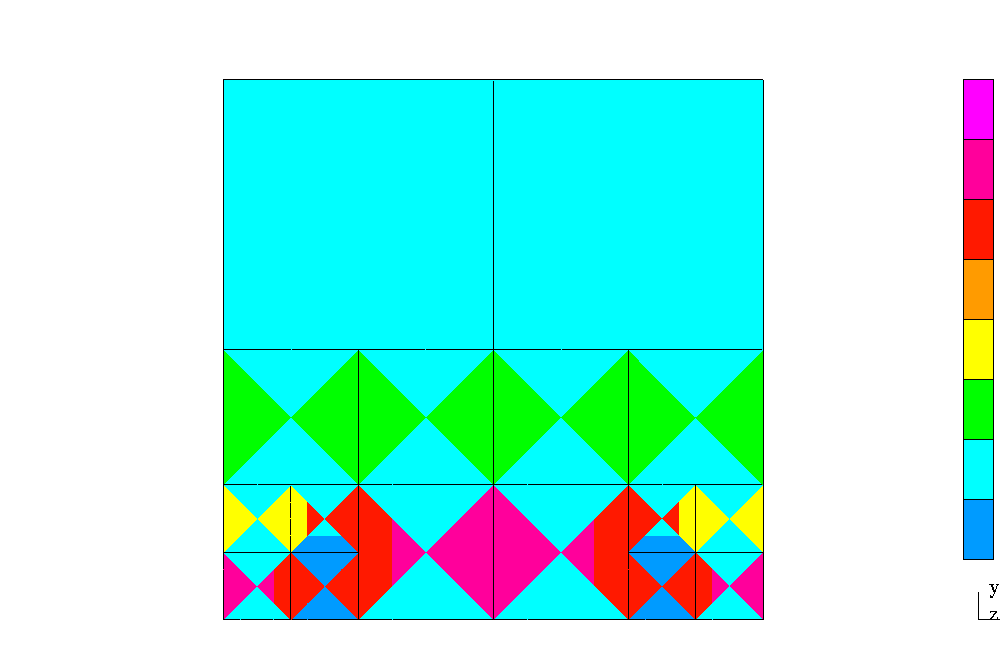
\includegraphics[scale=.15]{figs/mesh1.png}}
\subfigure{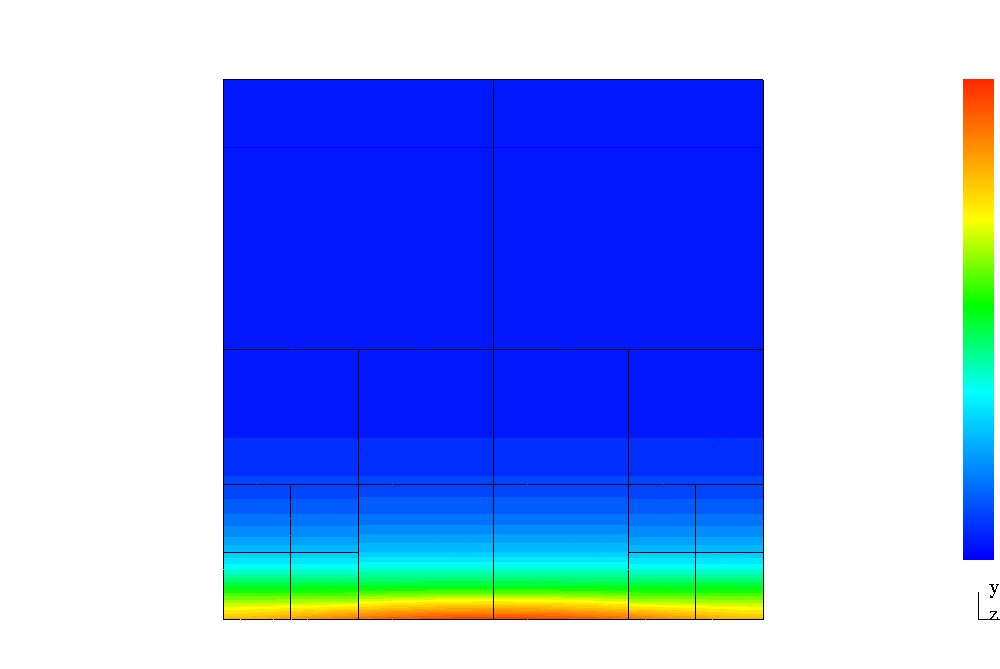
\includegraphics[scale=.15]{figs/sol1.png}}
\caption{The $v$ component of the optimal test function corresponding to flux $\widehat{u} = x(1-x)$ on the bottom side of a unit element for $\epsilon = 0.01$.}
\label{fig:boundaryTest}
\end{figure}
}
\frame{
\frametitle{Mesh-scaled test norms}
%To avoid boundary layers in the optimal test functions, we scale the $L^2$ contributions of $v$ by $C_v(K)$, such that, when transformed to the reference element, both $C_v(K)\|v\|^2$ and $\epsilon\|\grad v\|^2$ are of the same magnitude. Similarly, we scale the $L^2$ contributions of $\tau$ by $C_\tau(K)$ such that $\frac{C_\tau(K)}{\epsilon} \|\tau\|^2$ and $\|\div \tau\|^2$ are of the same magnitude as well.

Our test norm, as defined over a single element $K$, is now
\begin{align*}
\|\left(v,\tau\right)\|_{V,K}^2 = \min\left\{\frac{\epsilon}{|K|},1\right\}\|v\|^2 + \epsilon \|\grad v\|^2 + \|\beta \cdot \grad v\|^2 +&\\
\| \div \tau\|^2 + \min\left\{\frac{1}{\epsilon},\frac{1}{|K|}\right\}\|\tau\|^2&.
\end{align*}
%This modified test norm avoids boundary layers in the locally computed optimal test functions, but for adaptive meshes, provides additional stability in areas of heavy refinement, where the best approximation error tends to be large and stronger robustness is most necessary.  This leads to a test norm which produces easily approximable optimal test functions, but still provides \textit{asymptotically} the strongest test norm and tightest robustness results in the areas of highest error. 

}

\frame{
\frametitle{Dirichlet inflow boundary condition}
Standard choice of boundary condition: $u = u_0$ on inflow boundary $\Gamma_{\rm in}$. 
\begin{figure}[h!]
\centering
\subfigure[Primal problem]{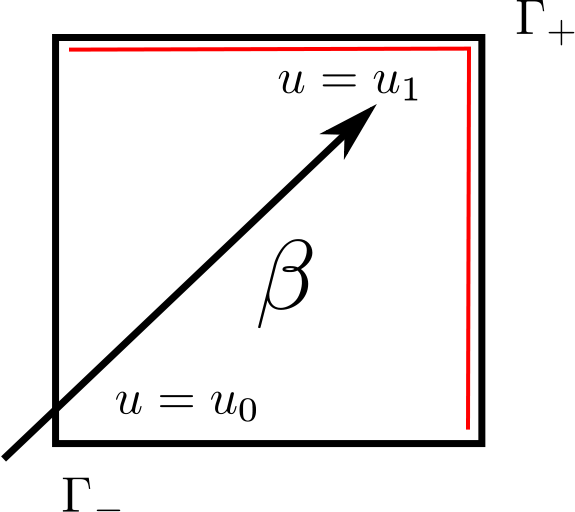
\includegraphics[scale=.2]{figs/primalDir.png}}
\subfigure[Adjoint problem]{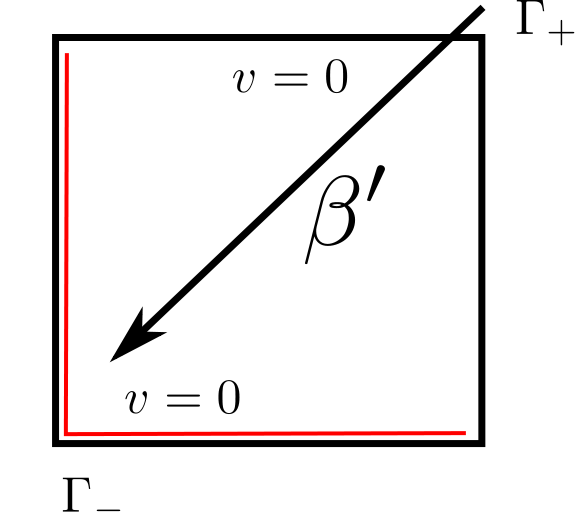
\includegraphics[scale=.2]{figs/adjointDir.png}}
\caption{For the standard Dirichlet inflow condition, the solution to the adjoint problem can develop strong boundary layers at the outflow of the adjoint problem. }
\end{figure}
}

\frame{
\frametitle{New inflow boundary condition on $\widehat{f}_n$}
Non-standard choice of boundary condition: $\widehat{f}_n = \beta_n u_0$ on $\Gamma_{\rm in}$. 
\begin{figure}[h!]
\centering
\subfigure[Primal problem]{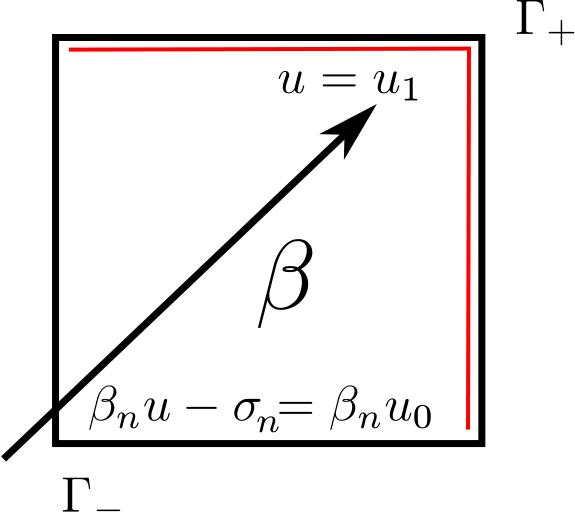
\includegraphics[scale=.2]{figs/primal.png}}
\subfigure[Adjoint problem]{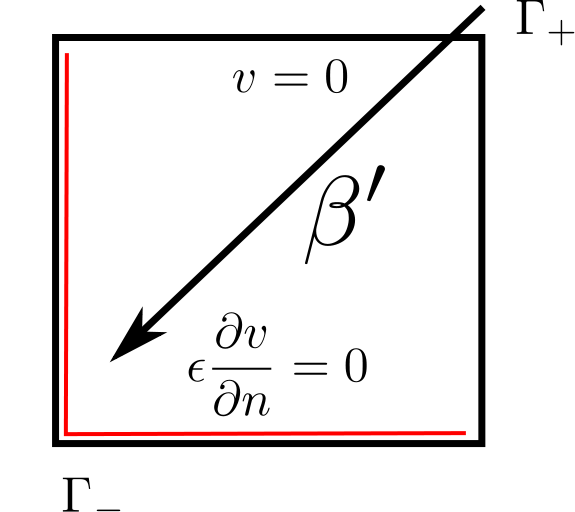
\includegraphics[scale=.2]{figs/adjoint.png}}
\caption{Under the new inflow condition, the wall-stop boundary condition is relaxed to a zero-stress condition at the outflow boundary of the adjoint problem.}
\end{figure}
}

\frame{
\frametitle{Test norms and adjoint solutions}
\begin{itemize}
\item Standard choice of boundary condition: $u = u_0$ on inflow boundary $\Gamma_{\rm in}$: induces boundary layers in adjoint problems.
\item Non-standard choice of boundary condition: $\widehat{f}_n = \beta_n u_0$ on $\Gamma_{\rm in}$: induces smoother adjoint problems.
\end{itemize}

\textbf{Intuition:} the effectiveness of DPG under a test norm is governed by how a \textbf{specific test norm} measures the \textbf{solutions of the adjoint problem}. 
}

\frame{
\frametitle{Erickson-Johnson model problem}

}

\frame{
\frametitle{Numerical experiments}

}
\frame{
More regularized solutions. 
}


\section{Proposed Work}
\frame{
\frametitle{DPG for nonlinear problems}

}
\frame{
\frametitle{Burgers' equation as an example}

}
\frame{
Results for Burgers

}

\frame{
\frametitle{Compressible Navier-Stokes equations}
\begin{align*}
\div \vecttwo{\rho u }{\rho v} &= 0\\
\div \left(\vecttwo{\rho u^2+p }{\rho u v} - \boldsymbol \sigma_{1}\right) &=0\\
\div \left(\vecttwo{\rho u v}{\rho v^2+p } - \boldsymbol \sigma_{2}\right) &=0\\
\div \left(\vecttwo{((\rho e)+p)u}{((\rho e)+p)v} - \boldsymbol\sigma \mathbf{u} + \vec{q}\right) &=0\\
\frac{1}{2\mu} \boldsymbol \sigma - \frac{\lambda}{4\mu (\mu + \lambda)} { \rm tr}(\boldsymbol \sigma) \boldsymbol I &= \grad \mathbf{u} - \Reyn \, {\boldsymbol \omega}\\
\frac{1}{\kappa}\vec{q} &= \grad T
\end{align*}
}
\frame{
$\boldsymbol\sigma$ is a Newtonian fluid $\sigma_{ij} = \mu(u_{i,j} + u_{j,i}) + \lambda u_{k,k} \delta_{ij}$.
%We can invert the stress tensor under isotropic and plane strain assumptions to get
\[
\frac{1}{2}\left(\grad  U + \grad ^T  U\right) = \frac{1}{2\mu} \sigma_{ij} - \frac{\lambda}{4\mu (\mu + \lambda)} \sigma_{kk}\delta_{ij}
\]
We also have
\[
\frac{1}{2}\left(\grad  U + \grad ^T  U\right) = \grad  U - \boldsymbol \omega
\]
%where $\boldsymbol \omega$ is the antisymmetric part of the infinitesimal strain tensor:
%\[
%\boldsymbol \omega = \frac{1}{2}\left(\grad  U - \grad ^T  U\right).
%\]
Our final form is
\begin{align*}
\grad  U - \boldsymbol \omega = \frac{1}{2\mu} \boldsymbol \sigma - \frac{\lambda}{4\mu (\mu + \lambda)} { \rm tr}(\boldsymbol \sigma) \boldsymbol I.
\end{align*}
Taking the antisymmetric part implicitly defines $\boldsymbol \omega$ to be the antisymmetric part of $\grad u$. 
}

\frame{
\frametitle{Extrapolation of test norms}
%\begin{columns}
%\begin{column}{.48\textwidth}
Convection-diffusion:
\begin{align*}
\div \left(\beta u - \sigma\right) &= f\\
\frac{1}{\epsilon}\sigma - \grad u &= 0.
\end{align*}
Navier-Stokes:%vectors of test functions  $v=\{v_1,v_2,v_3,v_4\}$, $W = \{\tau_1,\tau_2,\tau_3\}$. Similarly, we group our Eulerian and stress variables into the vector variables $U$ and $\Sigma$.  $R_{\rm Euler}(U,\Sigma)$ and $R_{\rm visc}(U,\Sigma)$ are Eulerian and viscous nonlinear residuals, our formulation for the linearized Navier-Stokes equations can be written as
\begin{align*}
\div \left(A_{\rm Euler}U - A_{\rm visc}\Sigma\right) &= R_{\rm Euler}(U,\Sigma)\\
E_{\rm visc} \Sigma - \grad U &= R_{\rm visc}(U,\Sigma)
\end{align*}
}

\frame{
Convection-diffusion:
\begin{align*}
\|\left(v,\tau\right)\|_{V,K}^2 =& \min\left\{\frac{\epsilon}{|K|},1\right\}\|v\|^2 + \epsilon \|\grad v\|^2 + \|\beta \cdot \grad v\|^2 \\
&+\| \div \tau\|^2 + \min\left\{\frac{1}{\epsilon},\frac{1}{|K|}\right\}\|\tau\|^2.
\end{align*}

Navier-Stokes:
\begin{align*}
\|\left(V,W\right)\|_{V,K}^2 =& \min\left\{\frac{\Reyn}{|K|},1\right\}\|v\|^2 + \frac{1}{\Reyn} \|A_{\rm visc}^T\grad v\|^2 + \|A_{\rm Euler}^T \grad v\|^2 \\
& + \| \div W\|^2 + \min\left\{\Reyn,\frac{1}{|K|}\right\}\|E_{\rm visc}^T\tau\|^2.
\end{align*}
%An advantage of this extrapolation approach is that the incompletely parabolic nature of the Navier-Stokes equation is taken into account; there is no diffusive term present in the mass conservation equation, and the test norm reflects that by requesting only limited regularity of $v_1$.\footnote{The situation is analogous to using the full $H^1(\Oh)$ norm for the pure convection equation --- the optimal test norm $\nor{v}_V = \nor{\beta\cdot \grad v} + \nor{v}$ implies only streamline regularity, whereas taking $\nor{v}_V = \nor{\grad v} + \nor{v}$ implies stronger regularity on the test space $V$ than the graph norm. Consequently, convergence is suboptimal for DPG applied to the convection problem under the $H^1(\Oh)$ test norm.}
%\end{column}
%\end{columns}
}
\frame{
\frametitle{Carter plate and Boundary conditions}

\begin{figure}[!h]
\centering
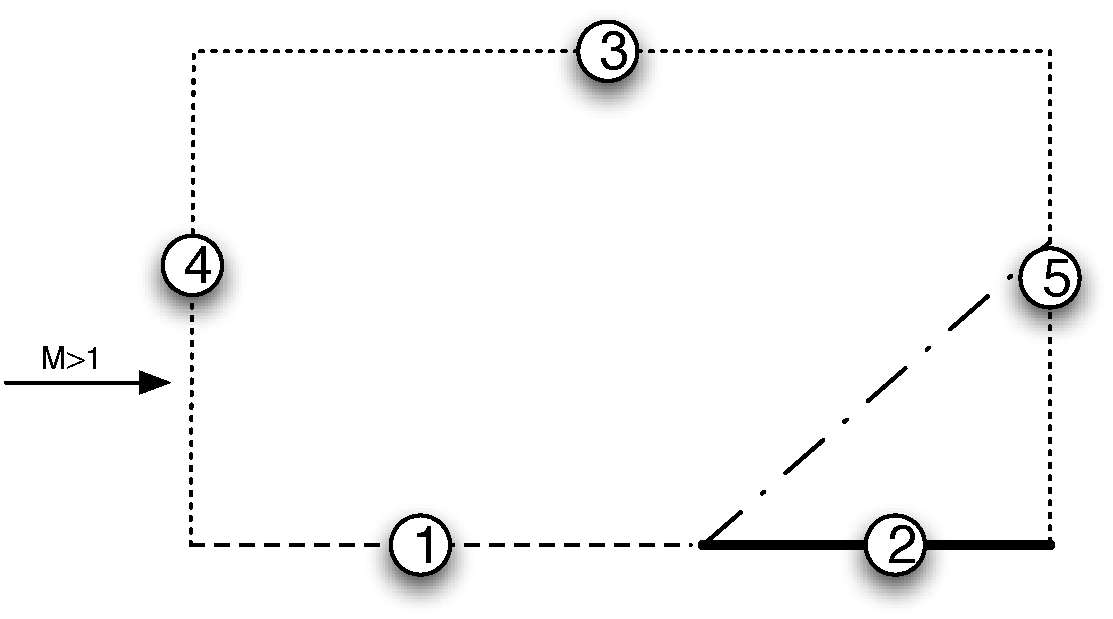
\includegraphics[scale=.35]{figs/flat_plate_BCs.pdf}
\caption{Carter flat plate problem.}
\end{figure}
\begin{itemize}
\item{} Inflow and stress boundary conditions, momentum flux boundary conditions. 
\item{} No outflow condition set.
\end{itemize}
}
\frame{
\frametitle{Refinement level 0}
\begin{figure}
\subfigure[$u_1$]{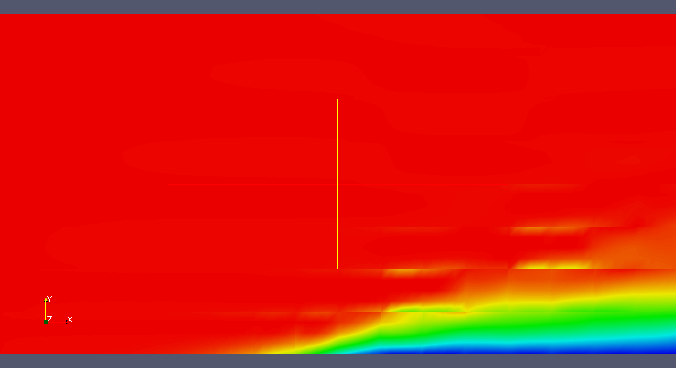
\includegraphics[scale = .23]{figs/Re1000p2/u10.png}}
\subfigure[$T$]{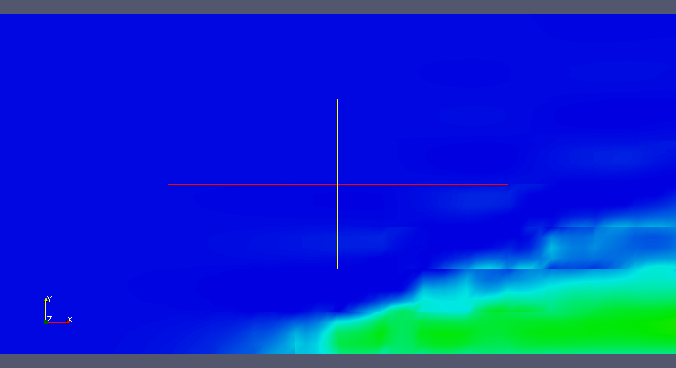
\includegraphics[scale = .23]{figs/Re1000p2/T0.png}}
\subfigure{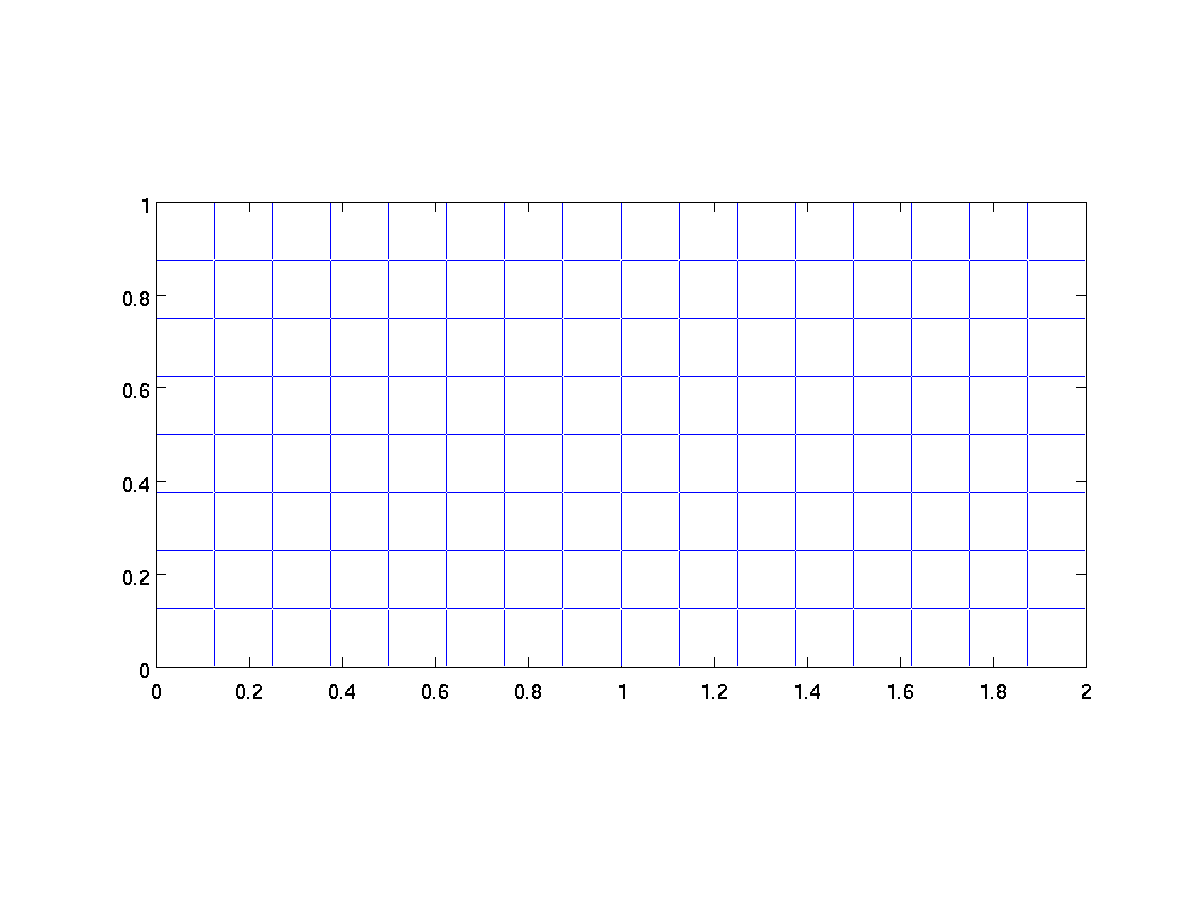
\includegraphics[scale = .35]{figs/Re1000p2/mesh0.png}}
\end{figure}
}
\frame{
\frametitle{Refinement level 1}
\begin{figure}
\subfigure[$u_1$]{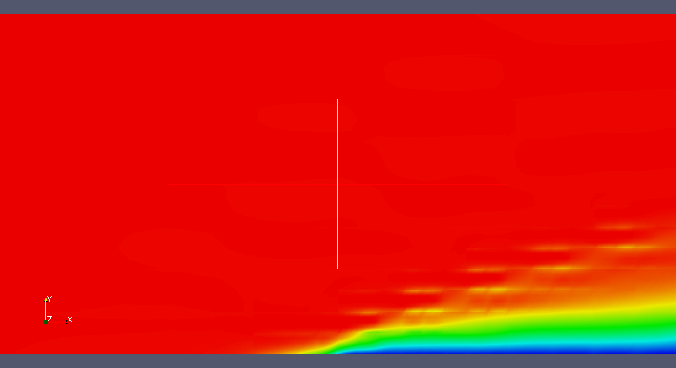
\includegraphics[scale = .23]{figs/Re1000p2/u11.png}}
\subfigure[$T$]{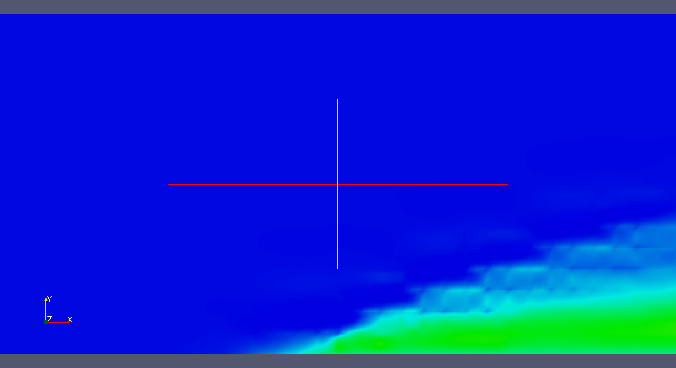
\includegraphics[scale = .23]{figs/Re1000p2/T1.png}}
\subfigure{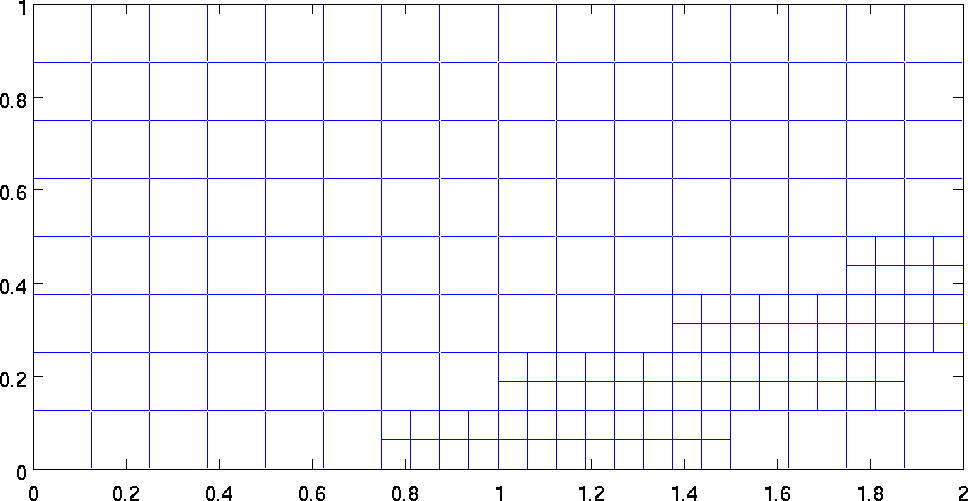
\includegraphics[scale = .35]{figs/Re1000p2/mesh1.png}}
\end{figure}
}
\frame{
\frametitle{Refinement level 2}
\begin{figure}
\subfigure[$u_1$]{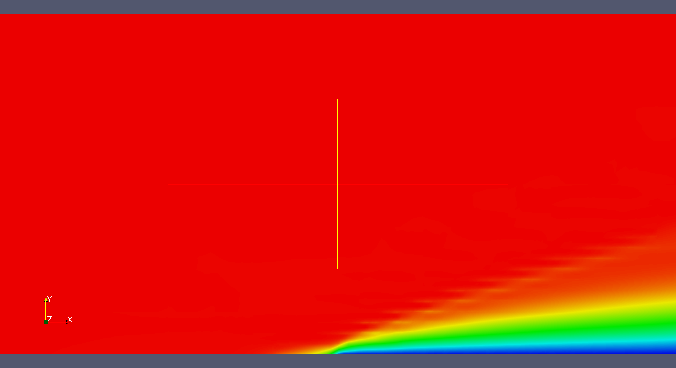
\includegraphics[scale = .23]{figs/Re1000p2/u12.png}}
\subfigure[$T$]{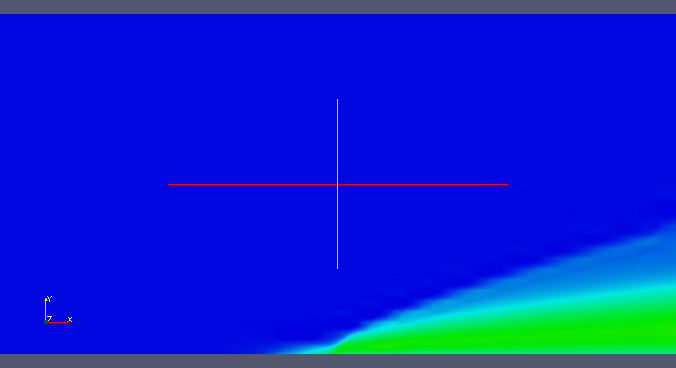
\includegraphics[scale = .23]{figs/Re1000p2/T2.png}}
\subfigure{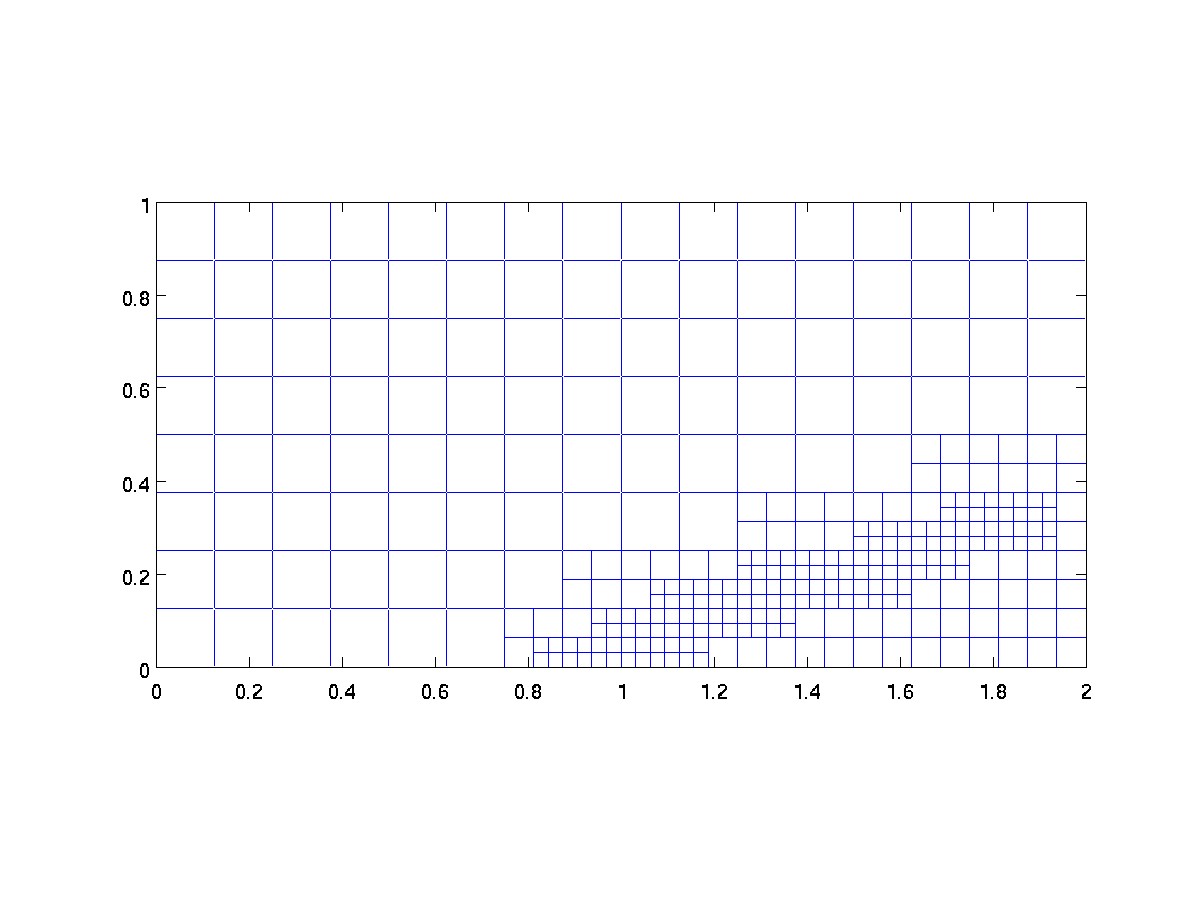
\includegraphics[scale = .35]{figs/Re1000p2/mesh2.png}}
\end{figure}
}
\frame{
\frametitle{Refinement level 3}
\begin{figure}
\subfigure[$u_1$]{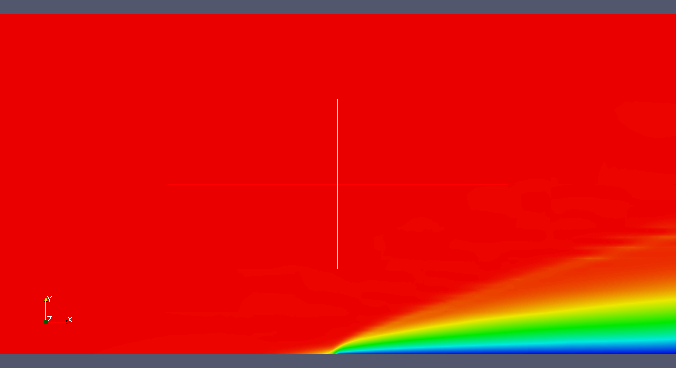
\includegraphics[scale = .23]{figs/Re1000p2/u13.png}}
\subfigure[$T$]{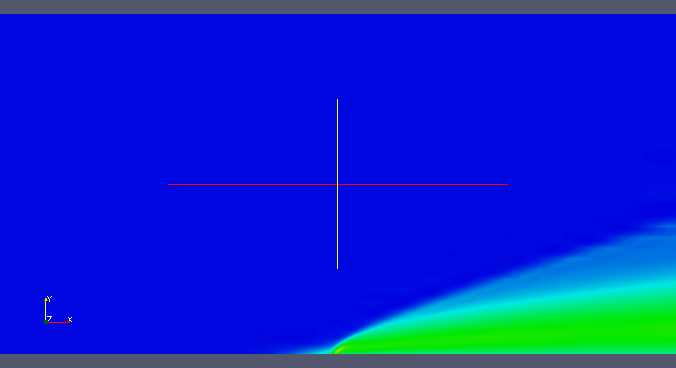
\includegraphics[scale = .23]{figs/Re1000p2/T3.png}}
\subfigure{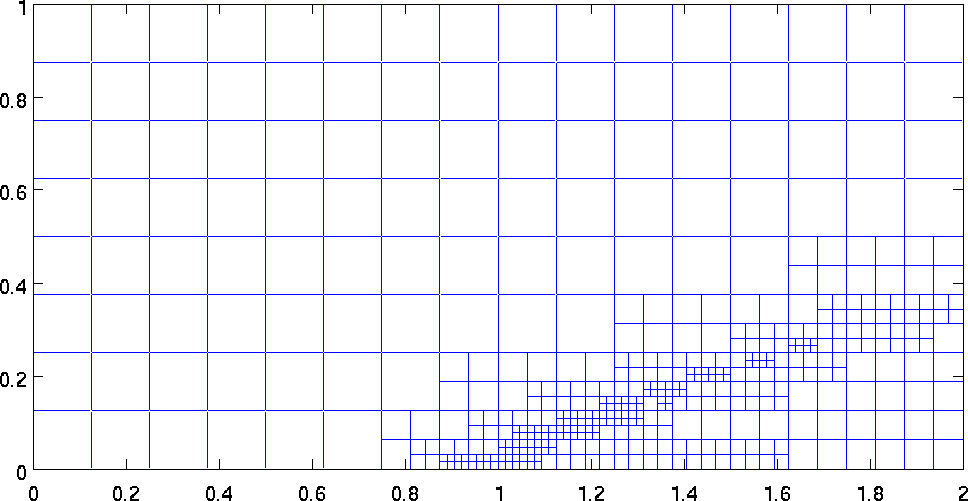
\includegraphics[scale = .35]{figs/Re1000p2/mesh3.png}}
\end{figure}
}
\frame{
\frametitle{Refinement level 4}
\begin{figure}
\subfigure[$u_1$]{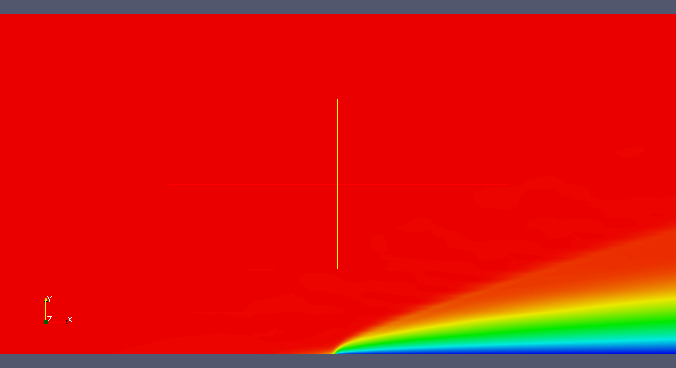
\includegraphics[scale = .23]{figs/Re1000p2/u14.png}}
\subfigure[$T$]{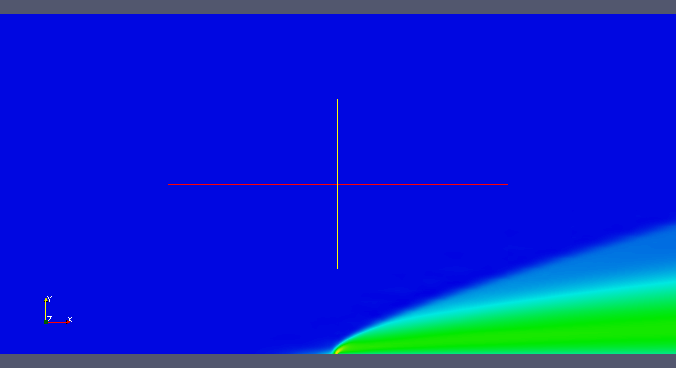
\includegraphics[scale = .23]{figs/Re1000p2/T4.png}}
\subfigure{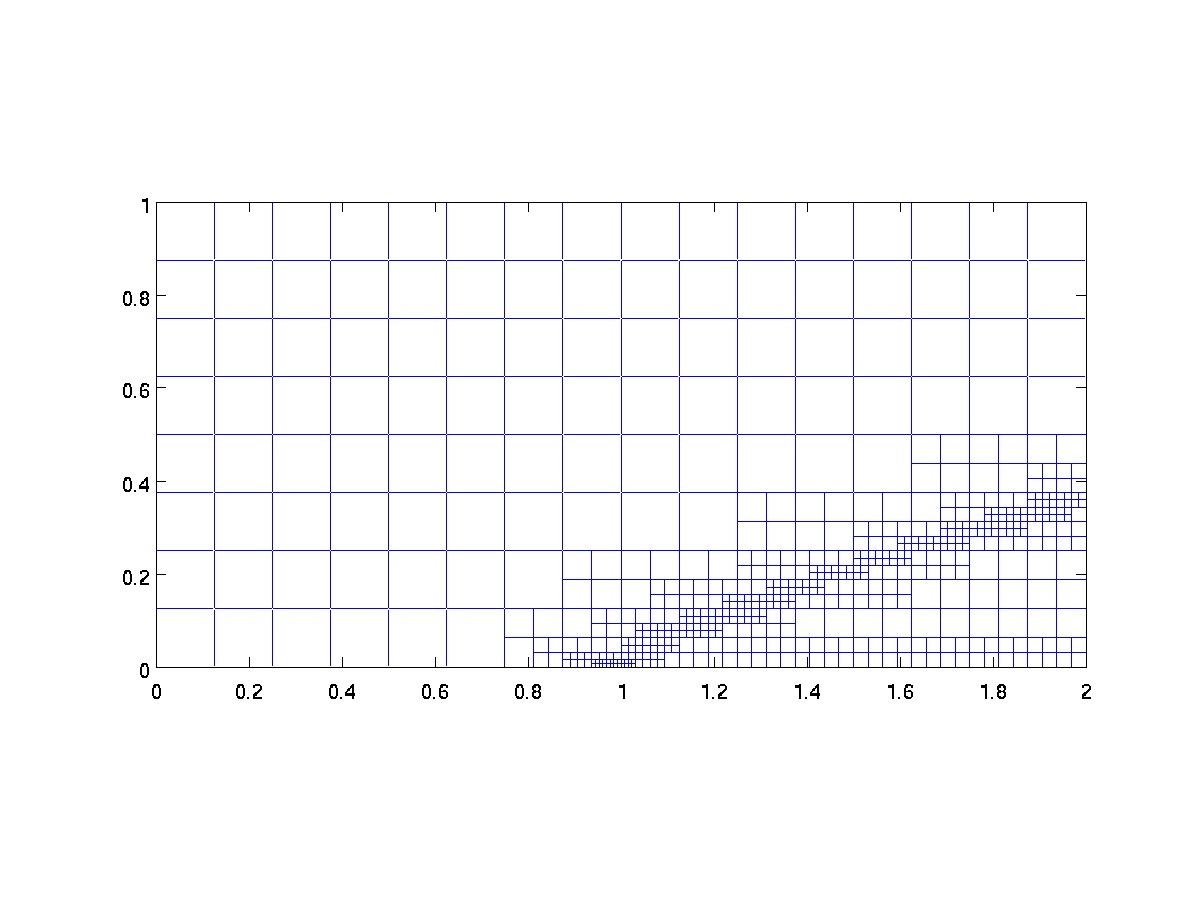
\includegraphics[scale = .35]{figs/Re1000p2/mesh4.png}}
\end{figure}
}
\frame{
\frametitle{Refinement level 5}
\begin{figure}
\subfigure[$u_1$]{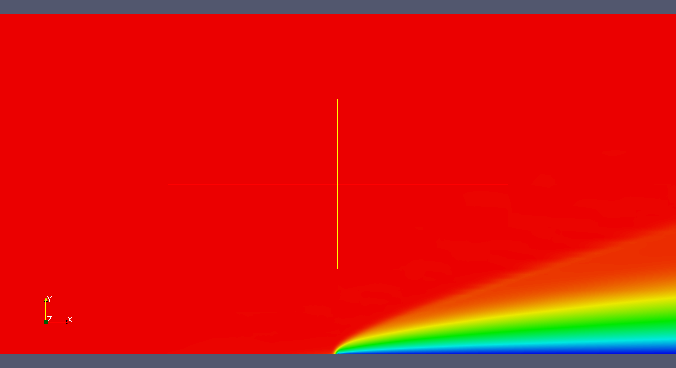
\includegraphics[scale = .23]{figs/Re1000p2/u15.png}}
\subfigure[$T$]{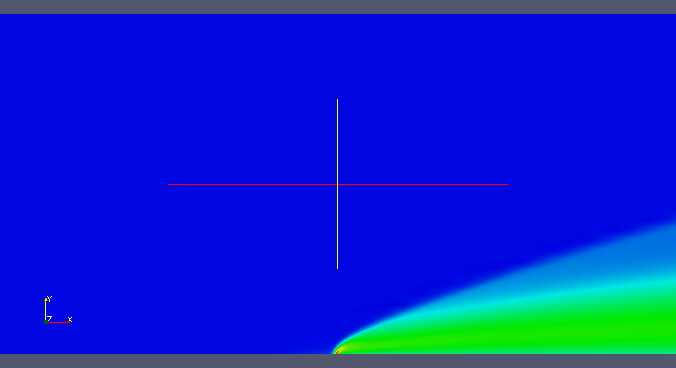
\includegraphics[scale = .23]{figs/Re1000p2/T5.png}}
\subfigure{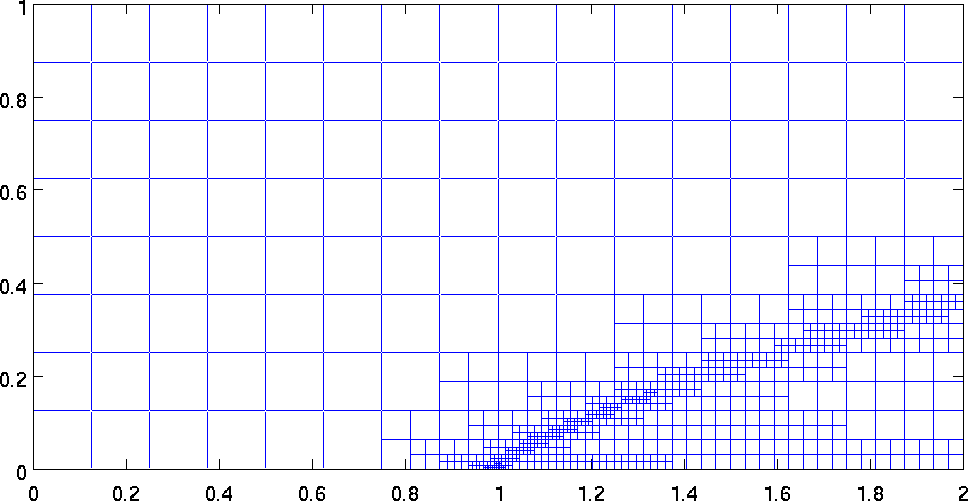
\includegraphics[scale = .35]{figs/Re1000p2/mesh5.png}}
\end{figure}
}
\frame{
\frametitle{Refinement level 6}
\begin{figure}
\subfigure[$u_1$]{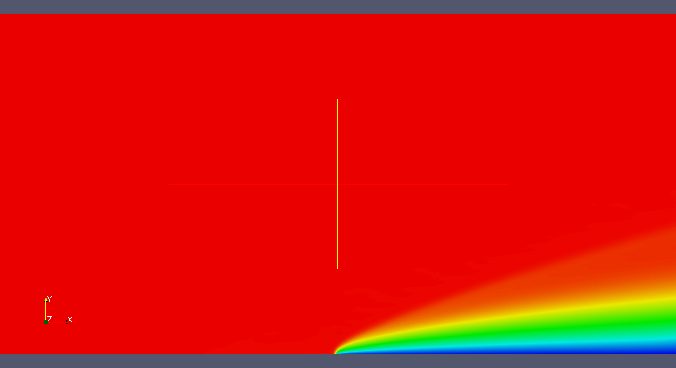
\includegraphics[scale = .23]{figs/Re1000p2/u16.png}}
\subfigure[$T$]{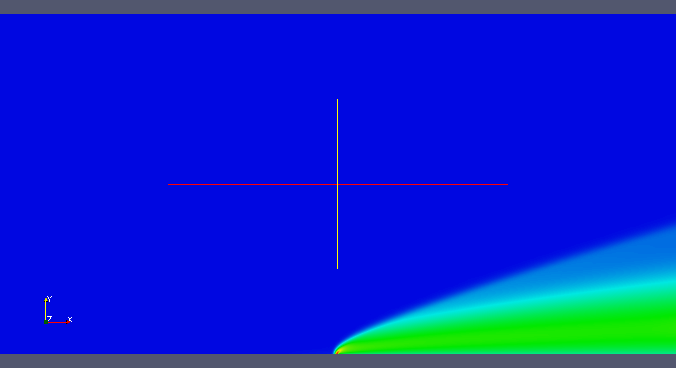
\includegraphics[scale = .23]{figs/Re1000p2/T6.png}}
\subfigure{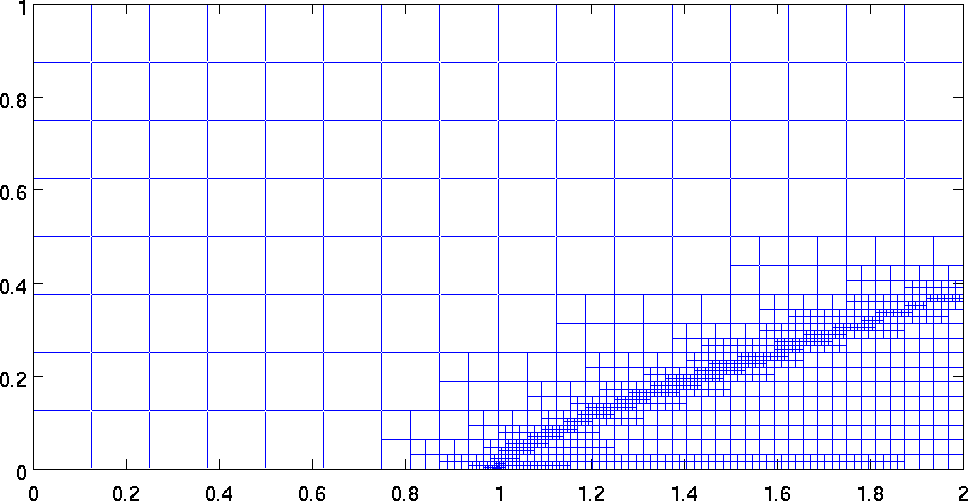
\includegraphics[scale = .35]{figs/Re1000p2/mesh6.png}}
\end{figure}
}

\frame{
\frametitle{Proposed work: Area A}

}
\frame{
\frametitle{Proposed work: Area B}

}
\frame{
\frametitle{Proposed work: Area C}

}
\end{document}
